%% LyX 2.3.6.2 created this file.  For more info, see http://www.lyx.org/.
%% Do not edit unless you really know what you are doing.
\documentclass[sigconf,nonacm]{acmart}
\usepackage[utf8]{inputenc}
\setcounter{secnumdepth}{3}
\setcounter{tocdepth}{3}
\usepackage{array}
\usepackage{mathtools}
\usepackage{graphicx}
\ifx\hypersetup\undefined
  \AtBeginDocument{%
    \hypersetup{unicode=true}
  }
\else
  \hypersetup{unicode=true}
\fi

\makeatletter

%%%%%%%%%%%%%%%%%%%%%%%%%%%%%% LyX specific LaTeX commands.
%% Because html converters don't know tabularnewline
\providecommand{\tabularnewline}{\\}

%%%%%%%%%%%%%%%%%%%%%%%%%%%%%% User specified LaTeX commands.
\usepackage{pgfplots}
\usepackage{subcaption}
\usepackage{adjustbox}
\usepackage{url}
%\usepackage{minted}


%\DeclareUnicodeCharacter{2212}{}
\usepgfplotslibrary{groupplots,dateplot}
\usetikzlibrary{
    patterns,
    chains,
    backgrounds,
    calc,
    shadings,
    shapes.arrows,
    arrows,
    shapes.symbols,
    shadows,
    positioning,
    decorations.markings,
    backgrounds,
    arrows.meta,
    external
}
\usepackage{array}


\pgfplotsset{compat=newest}

\newcommand{\code}[1]{\texttt{#1}}

\newif\iffinal

\iffinal
  \newcommand{\maxx}[1]{}
  \newcommand{\ryan}[1]{}
  \newcommand{\todo}[1]{}
\else
  \newcommand{\maxx}[1]{{\textcolor{red}{ Max: #1 }}}
  \newcommand{\ryan}[1]{{\textcolor{magenta}{ Ryan: #1 }}}
  \newcommand{\todo}[1]{{\textcolor{blue}{ TODO: #1 }}}
\fi

\makeatother

\begin{document}
\title{Ultrafast focus detection using multi-scale histologic features}
\author{Maksim Levental}
\affiliation{\institution{University of Chicago}}
\author{Ryan Chard}
\affiliation{\institution{Argonne National Laboratory}}
\author{Gregg A. Wildenberg}
\affiliation{\institution{University of Chicago}}
\begin{abstract}
We present a fast out-of-focus detection algorithm for electron microscopy
images collected serially. Such images are collected for the purposes
of post-processing tasks such as montaging, alignment, and image segmentation.
Such an algorithm is necessitated by recent increases in collection
rates owing to advances in microscopy technology. Our technique adapts
classical computer vision and is based on detecting various fine-grained
histologic features. We further exploit the inherent parallelism in
the technique by employing GPGPU primitives in order to accelerate
characterization. Tests are performed that demonstrate faster than
real time detection of out-of-focus conditions. \textless We also
deploy to funcX something something\textgreater . We discuss extensions
that enable scaling out to support multi-beam microscopes and integration
with existing focus systems for purposes of implementing auto-focus.
\end{abstract}
\maketitle

\section{Introduction}

\label{sec:intro}

Advancements in the automation of serial scanning electron microscopy
(SEM) impose a regime where thousands, if not tens of thousands, of
images can now be automatically collected by researchers. \todo{\textless bio
use cases\textgreater} This puts greater demand on conventional
auto-focus algorithms for ensuring each image is in focus, as an alternative
to the user manually evaluating each image by eye. Without such algorithms,
critical bottlenecks are created where the user is forced to reacquire
individual, deficient (out-of-focus), images and manually reinsert
them into the sequence of thousands of other images already acquired.
This is an onerous task which requires taking into account alignment
and boundary overlap. Furthermore, failure to quickly identify and
reacquire deficient images negatively impacts the accuracy of downstream,
post-processing; for example 2D montaging, 3D alignment, or automatic
segmentation pipelines. While many microscopes have builtin auto-focus
algorithms, these often fail to achieve acceptable accuracy due to
intrinsic mediating factors (e.g. stage drift) and extrinsic mediating
factors (e.g. sample artifacts, non-uniformity in the sample).

Auto-focus technology is a critical component of many imaging systems;
from consumer cameras (for purposes of convenience) to industrial
inspection tools to scientific instrumentation. Such technology is
typically either active or passive; active methods exploit some auxiliary
device or mechanism to measure the distance of the optics from the
scene, while passive methods analyze the definition of sharpness of
an image by virtue of some proxy measure. Here we focus on passive
methods, as we explicitly aim to augment existing microscopy equipment
without the need for costly and complex retrofitting.

Passive proxies for the degree-of-focus (DOF) include the energy of
the Laplacian, discrete cosine transform, or weighted histogram of
an image; for effecting a high DOF a search can be performed. When
used as a component of an auto-focus system (as opposed to OOF detection
system) all such passive methods are unsuitable for the purpose of
real-time (or even near-real-time) characterization of DOF due to
their long scanning times (multiple images need to be collected at
potentially different depths). As our method currently aims only to
detect OOF events we do not consider or implement any focus search
techniques (but do describe plans for such future work).

To overcome these challenges, thereby ensuring that images are faithfully
acquired, we propose a method to evaluate image definition based multi-scale
histologic feature detection (MHFD). By multi-scale histologic feature
detection we mean the resolving and characterization of histological
structure at multiple length scales; for our particular use-case this
means structures ranging from cell walls to whole organelles. The
key insight being that the ability to resolve structure across the
range of feature scales is highly correlated with a high-definition,
i.e. in-focus, image.

Due to limitations of the extensibility of commercial microscopy equipment,
we do not aim here to directly implement auto-focusing. Rather than
focusing the microscope, as auto-focusing algorithms would, our algorithm
operates downstream of collection and reports out-of-focus (OOF) events
to the user. This enables the user to intervene and initiate reacquisition
protocols (on the microscope) before unknowingly proceeding with collecting
the next series of images or proceeding with downstream image processing
and analysis. This human-in-the-loop remediation protocol already
saves the user much wasted collection time and tedium in triaging
defective collection runs.

This rest of this article is organized as follows: section~\ref{sec:mhd}
describes our focus detection method in the abstract, section \ref{sec:implementation}
discusses optimizations made in order to achieve real-time performance
with our method, section \ref{sec:Evaluation} reports results of
evaluating our method on sequences of images collected at varying
focus depths, section \ref{sec:related} discusses related work and
how our work is distinct therefrom, and finally section \ref{sec:conclusion}
concludes with a discussion of future research.

\section{Significance to Neuroscience and Connectomics}

A fundamental goal of neuroscience is to map the anatomical wiring of the brain. Such an effort is difficult because currently electron microscopy, an imaging method traditionally limited to small 2D images, is the only imaging modality with sufficient resolution to directly visualize the connections, or synapses, between neurons. Recently, automated serial electron microscopy (‘connectomics’) has been developed where 1,000’s if not 10’s of thousands of individual 2D images are automatically acquired in series and then algorithmically aligned to produce a volumetric dataset. Such 3D datasets allow neuroscientists to follow the tortuous path neurons take through the brain to connect with each other. However, many of the steps to collecting 3D datasets for connectomics require manual inspection causing significant slowdowns in the rate in which datasets can be acquired. Such bottlenecks significantly impact the size of datasets that can be reasonably acquired and studied. Without high fidelity automation to the imaging pipeline, the field of connectomics will fail to advance and realize its full potential.

One part of the imaging pipeline we sought to improve through automation is automatically ensuring that images acquired by the electron microscope are in-focus. and status of the microscope. While perhaps a small step in the process, focus detection it is nevertheless an extremely critical step. Without properly focused images, all downstream computational steps (i.e. 2D tile montaging, 3D alignment, automatic segmentation) will fail. Furthermore, because imaging sections requires loading and unloading sets of ~100-200 sections at a time, a failure manually flag an out of focus image in real time causes significant delays in having to reload the sample set, find the desired field of view, reacquire, and insert that new image into the image stack. Finally, advances in electron microscopes have pushed the rate that images can be acquired (e.g. ~10 Tbs/24hr) further necessitating the need for high throughput automation that ensures images are acquired in focus in order for downstream computational pipelines and ultimately analysis of biological results to keep pace with data acquisition. While many electron microscopes have built-in automatic focus algorithms that attempt to focus the microscope before image acquisition, blurry images still occur at about 1-10\% of the time depending on the quality of the tissue sections being imaged. Our proposed solution is to have a second pass analysis of the blurriness of the image after they are acquired using machine learning methods to flag images that failed to pass the initial autofocus step.  


\section{Multi-scale Histologic Feature Detection\label{sec:mhd}}

\subsection{Scale-space}

We base our multi-scale histologic feature detection on classic scale-space
representations of signals. We give a brief overview (a more comprehensive
discussion is available \citet{Lindeberg2004FeatureDW}) and describe
our adaptation.

The fundamental principle of scale-space feature detection is that
natural images possess structure at multiple scales and that features
at a particular scale can be characterized in isolation of features
at other scales. Typically, characterization is effected by convolution
with a filter that satisfies the constraints of non-enhancement of
local extrema, scale invariance and rotational invariance (along with
some others \citet{duits2004axioms}). One such filter \citet{koenderink1984structure}
is the symmetric, mean zero, two dimensional, Gaussian filter 
\[
G(x,y,\sigma)\coloneqq\frac{1}{2\pi\sigma^{2}}e^{-\frac{x^{2}+y^{2}}{2\sigma^{2}}}
\]
Thus, define the scale-space representation $L(x,y,t)$ of an image
$I(x,y)$ to be the convolution of that image with a mean zero Gaussian
filter: 
\[
L(x,y,t)\coloneqq G(x,y,t)*I(x,y)
\]
where $t$ determines the \textit{scale} of $L(x,y,t)$. $L(x,y,t)$
has the interpretation that image structures of scale smaller than
$\sqrt{t^{2}}=t$ have been removed due to blurring. This is due to
the fact that the variance of the Gaussian filter is $t^{2}$ and
features of this scale are therefore ``beneath the noise floor''
of the filter or, in effect, suppressed by filtering procedure. A
corollary is that features with approximate length scale $t$ will
have maximal response upon being filtered by $G(x,y,t)$; for $t'<t$
smaller length scale features will dominate the response and for $t''>t$,
as already mentioned, the response will have been suppressed. Hence,
at various scales we can use linear and non-linear combinations of
space derivatives $\partial_{x},\partial_{y}$ and derivatives in
scale $\partial_{t}$ to construct scale-invariant feature detectors;
such feature detectors detect features such as corners, edges, and
ridges. For example, the critical points in $t$ 
\begin{equation}
\partial_{t}\nabla^{2}L\coloneqq\partial_{t}\left(\partial_{x}^{2}+\partial_{y}^{2}\right)L\label{eqn:blobdetector}
\end{equation}
correspond to uniform region (otherwise known as blobs) detectors.

\subsection{Multi-scale Histologic Feature Detection}

\label{sec:implementation}

\begin{figure}
\centering \begin{subfigure}[b]{0.5\textwidth} \centering 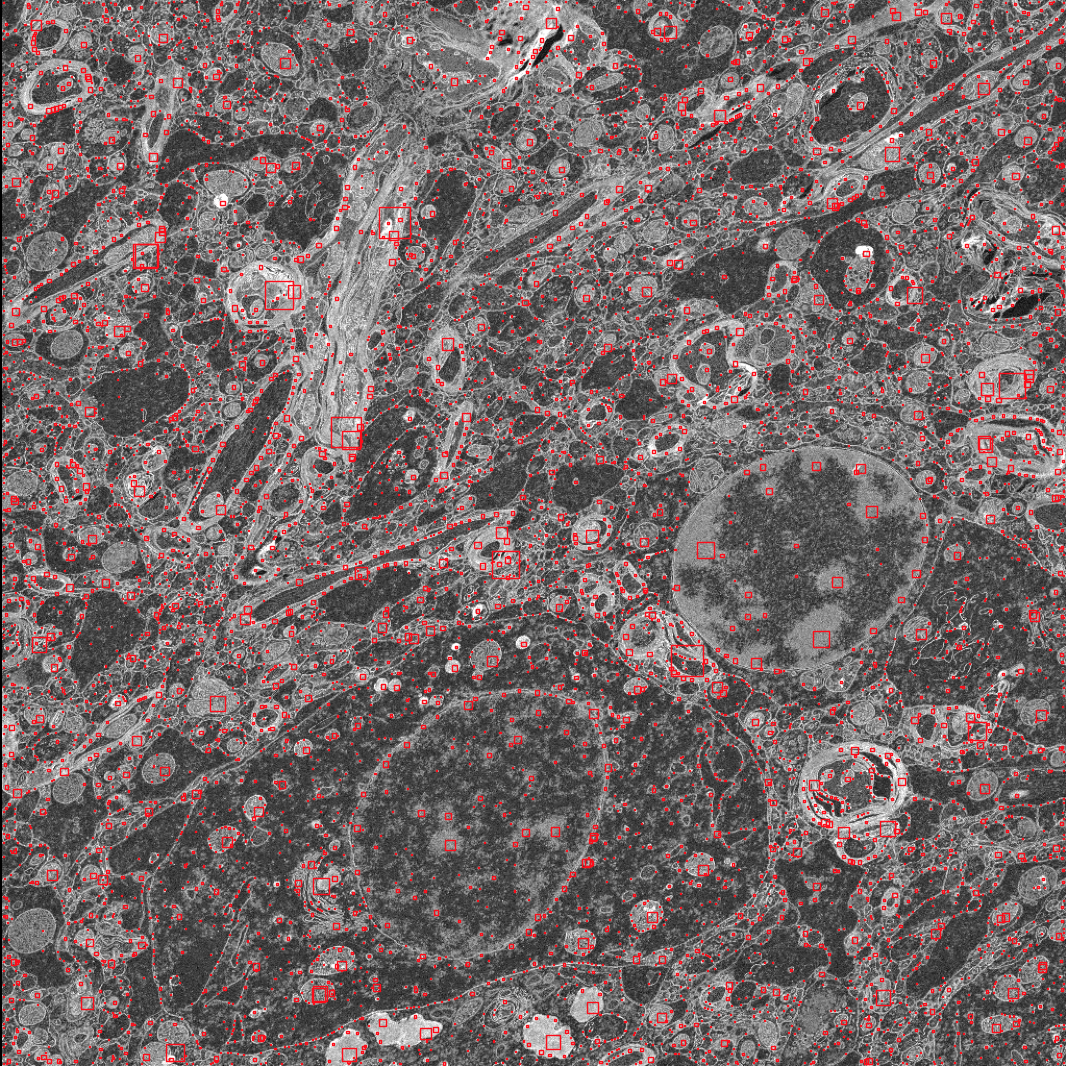
\includegraphics[width=1\linewidth]{in_focus}
\caption{Histologic features of an in-focus section.}
\label{subfig:infocus} \end{subfigure} 

\medskip{}
\begin{subfigure}[b]{0.5\textwidth} \centering 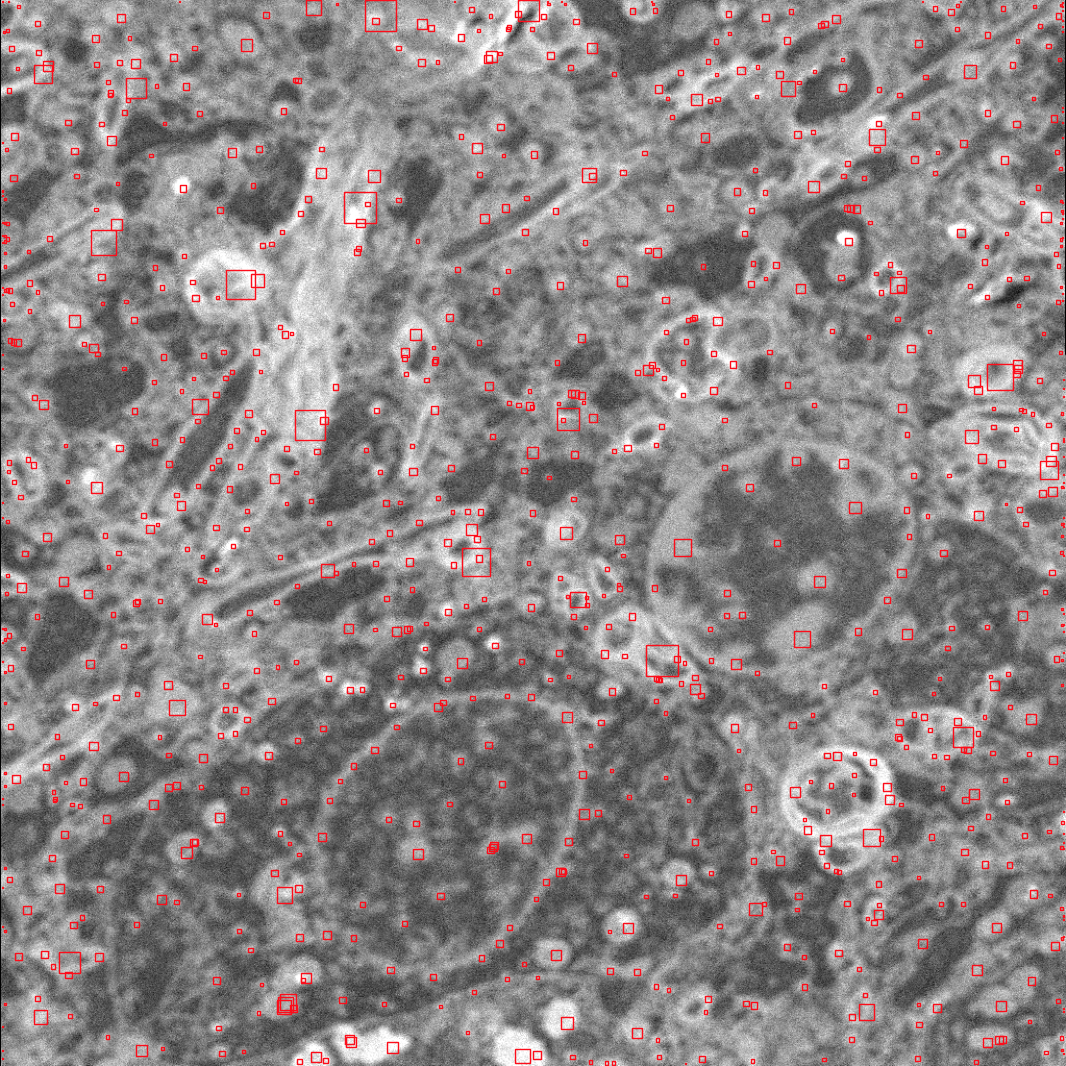
\includegraphics[width=1\linewidth]{out_of_focus}
\caption{Histologic features of an out-of-focus section.}
\label{subfig:outoffocus} \end{subfigure} \caption{Comparison of sections with histologic feature recognition as a function
of focal depth.}
\label{fig:histfeatsimages} 
\end{figure}

We propose to use feature detection as a proxy for DOF, reasoning
that the quantity of features detected is positively correlated with
DOF (see figure \ref{fig:histfeatsimages}). To this end, we develop
a feature detector based on eqn. \ref{eqn:blobdetector} but optimized
for latency (rather than for accuracy). In order to verify our hypothesis
we compare the number of histologic features detected as a function
of absolute deviation from in-focus ($\lvert f-f'\rvert$ where $f'$
is the correct focal depth) for a series of sections with known focal
depth (see figure \ref{subfig:degreeoofcurve}). We observe a very
strong log-linear relationship (see figure \ref{subfig:degreeooffit}).
Fitting such a log-linear relationship produces a line with $r=-0.9754$,
confirming our hypothesis that quantity of histologic features detected
is a good proxy measure for DOF.

\begin{figure}
\centering \begin{subfigure}[b]{0.5\textwidth} \centering % This file was created by tikzplotlib v0.9.8.
\begin{tikzpicture}[trim axis left,trim axis right]

\definecolor{color0}{rgb}{0.12156862745098,0.466666666666667,0.705882352941177}

\begin{axis}[
scaled y ticks=base 10:-3,
legend cell align={left},
legend style={fill opacity=0.8, draw opacity=1, text opacity=1, draw=white!80!black},
tick align=outside,
tick pos=left,
% title={Feature count vs. OOF},
x grid style={white!69.0196078431373!black},
xlabel={Degree of OOF},
xmin=-1.09892007559144e-06, xmax=2.31000189170211e-05,
xtick style={color=black},
xmajorgrids,
ymajorgrids,
y grid style={white!69.0196078431373!black},
ylabel={\# features},
ymin=99.9931235536055, ymax=9059.85673521721,
ytick style={color=black},
% y tick label style={/pgf/number format/sci}
]
\addplot [draw=color0, fill=color0, forget plot, mark=*, mark size=1, only marks, mark options={solid,fill opacity=0}]
table{%
x  y
2.89713740402389e-08 7023
1.79997717738205e-05 977
9.99997577071001e-06 1882
2.00011560321043e-06 6755
6.00014606118044e-06 4607
1.20001917481398e-05 2045
2.19998022317905e-05 743
1.99991485475958e-06 6791
3.99993008374979e-06 5606
5.99994531274e-06 3664
1.80000366866596e-05 899
2.00000519156498e-05 798
8.00016129016978e-06 3590
1.000017651916e-05 2672
1.400020697713e-05 1644
1.99997870028003e-05 874
7.99996054173021e-06 2513
1.40000062286896e-05 1233
1.60002222061202e-05 1185
1.19999909997002e-05 1419
1.60000214576702e-05 1056
4.00013083219977e-06 5610
2.20000671446296e-05 728
1.400020697713e-05 1172
3.99993008374979e-06 6308
7.99996054173021e-06 2688
9.99997577071001e-06 2037
1.03169680003984e-09 7000
1.000017651916e-05 1794
2.19998022317905e-05 741
1.99991485475958e-06 6987
5.99994531274e-06 4299
1.40000062286896e-05 1291
1.80000366866596e-05 988
2.00011560321043e-06 6389
4.00013083219977e-06 4785
6.00014606118044e-06 3080
8.00016129016978e-06 2329
1.20001917481398e-05 1472
1.60002222061202e-05 995
1.79997717738205e-05 882
1.19999909997002e-05 1595
1.60000214576702e-05 1103
2.00000519156498e-05 847
2.20000671446296e-05 781
1.99997870028003e-05 798
1.14187389609749e-07 8645
1.74120792746993e-06 8487
4.00013083219977e-06 5997
2.19998022317905e-05 831
1.99991485475958e-06 8516
3.99993008374979e-06 6280
9.99997577071001e-06 2037
1.80000366866596e-05 1004
6.00014606118044e-06 3510
8.00016129016978e-06 2658
1.20001917481398e-05 1517
1.60002222061202e-05 1095
7.99996054173021e-06 2740
2.00000519156498e-05 888
1.000017651916e-05 1958
1.79997717738205e-05 1022
1.99997870028003e-05 899
1.19999909997002e-05 1634
1.40000062286896e-05 1333
1.60000214576702e-05 1118
1.400020697713e-05 1253
5.99994531274e-06 3899
};
% \addplot [semithick, red]
% table {%
% 1.03169680003984e-09 8652.59020741432
% 2.89713740402389e-08 8621.47458132233
% 1.14187389609749e-07 8527.26131703851
% 1.74120792746993e-06 6913.51092038955
% 1.99991485475958e-06 6686.69355019204
% 1.99991485475958e-06 6686.69355019204
% 1.99991485475958e-06 6686.69355019204
% 2.00011560321043e-06 6686.52046851991
% 2.00011560321043e-06 6686.52046851991
% 3.99993008374979e-06 5166.70076818288
% 3.99993008374979e-06 5166.70076818288
% 3.99993008374979e-06 5166.70076818288
% 4.00013083219977e-06 5166.56703075379
% 4.00013083219977e-06 5166.56703075379
% 4.00013083219977e-06 5166.56703075379
% 5.99994531274e-06 3992.22674518632
% 5.99994531274e-06 3992.22674518632
% 5.99994531274e-06 3992.22674518632
% 6.00014606118044e-06 3992.1234084266
% 6.00014606118044e-06 3992.1234084266
% 6.00014606118044e-06 3992.1234084266
% 7.99996054173021e-06 3084.72952084398
% 7.99996054173021e-06 3084.72952084398
% 7.99996054173021e-06 3084.72952084398
% 8.00016129016978e-06 3084.6496741889
% 8.00016129016978e-06 3084.6496741889
% 8.00016129016978e-06 3084.6496741889
% 9.99997577071001e-06 2383.52098318378
% 9.99997577071001e-06 2383.52098318378
% 9.99997577071001e-06 2383.52098318378
% 1.000017651916e-05 2383.45928695194
% 1.000017651916e-05 2383.45928695194
% 1.000017651916e-05 2383.45928695194
% 1.19999909997002e-05 1841.70840227035
% 1.19999909997002e-05 1841.70840227035
% 1.19999909997002e-05 1841.70840227035
% 1.20001917481398e-05 1841.66073058486
% 1.20001917481398e-05 1841.66073058486
% 1.20001917481398e-05 1841.66073058486
% 1.40000062286896e-05 1423.05851843724
% 1.40000062286896e-05 1423.05851843724
% 1.40000062286896e-05 1423.05851843724
% 1.400020697713e-05 1423.02168329095
% 1.400020697713e-05 1423.02168329095
% 1.400020697713e-05 1423.02168329095
% 1.60000214576702e-05 1099.57447357174
% 1.60000214576702e-05 1099.57447357174
% 1.60000214576702e-05 1099.57447357174
% 1.60002222061202e-05 1099.54601164414
% 1.60002222061202e-05 1099.54601164414
% 1.60002222061202e-05 1099.54601164414
% 1.79997717738205e-05 849.652567006649
% 1.79997717738205e-05 849.652567006649
% 1.79997717738205e-05 849.652567006649
% 1.80000366866596e-05 849.623544825807
% 1.80000366866596e-05 849.623544825807
% 1.80000366866596e-05 849.623544825807
% 1.99997870028003e-05 656.512899491502
% 1.99997870028003e-05 656.512899491502
% 1.99997870028003e-05 656.512899491502
% 2.00000519156498e-05 656.490474517362
% 2.00000519156498e-05 656.490474517362
% 2.00000519156498e-05 656.490474517362
% 2.19998022317905e-05 507.276978773357
% 2.19998022317905e-05 507.276978773357
% 2.19998022317905e-05 507.276978773357
% 2.20000671446296e-05 507.259651356497
% 2.20000671446296e-05 507.259651356497
% };
% \addlegendentry{\#features $\approx 8653.74e^{-128941.61x}$}
\end{axis}

\end{tikzpicture}

\caption{Number of histologic features as a function of absolute deviation
from focused ($\lvert f-f'\rvert$ where $f'$ is the correct focal
depth).}
\label{subfig:degreeoofcurve} \end{subfigure} 

\medskip{}
\begin{subfigure}[b]{0.5\textwidth} \centering % This file was created by tikzplotlib v0.9.8.
\begin{tikzpicture}[trim axis left,trim axis right]

\definecolor{color0}{rgb}{0.12156862745098,0.466666666666667,0.705882352941177}

\begin{axis}[
legend cell align={left},
legend style={fill opacity=0.8, draw opacity=1, text opacity=1, draw=white!80!black},
tick align=outside,
tick pos=left,
% title={Log feature count vs. OOF},
x grid style={white!69.0196078431373!black},
xlabel={Degree of OOF},
xmin=-1.09892007559144e-06, xmax=2.31000189170211e-05,
xtick style={color=black},
y grid style={white!69.0196078431373!black},
ylabel={log (\#features)},
xmajorgrids,
ymajorgrids,
ymin=6.26154869922026, ymax=9.1982215266363,
ytick style={color=black}
]
\addplot [draw=color0, fill=color0, forget plot, mark=*, only marks]
table{%
x  y
2.89713740402389e-08 8.85694575615902
1.79997717738205e-05 6.88448665204278
9.99997577071001e-06 7.54009032014532
2.00011560321043e-06 8.8180382503943
6.00014606118044e-06 8.43533216493592
1.20001917481398e-05 7.6231530684769
2.19998022317905e-05 6.61069604471776
1.99991485475958e-06 8.82335348511379
3.99993008374979e-06 8.63159273172473
5.99994531274e-06 8.20631072579402
1.80000366866596e-05 6.80128303447162
2.00000519156498e-05 6.68210859744981
8.00016129016978e-06 8.18590748148232
1.000017651916e-05 7.89058253465654
1.400020697713e-05 7.40488757561612
1.99997870028003e-05 6.77308037565554
7.99996054173021e-06 7.82923253754359
1.40000062286896e-05 7.11720550316434
1.60002222061202e-05 7.07749805356923
1.19999909997002e-05 7.25770767716004
1.60000214576702e-05 6.96224346426621
4.00013083219977e-06 8.63230599851674
2.20000671446296e-05 6.59030104819669
1.400020697713e-05 7.06646697013696
3.99993008374979e-06 8.74957394808293
7.99996054173021e-06 7.89655270164304
9.99997577071001e-06 7.61923341622681
1.03169680003984e-09 8.85366542803745
1.000017651916e-05 7.49220304261874
2.19998022317905e-05 6.60800062529609
1.99991485475958e-06 8.85180655855245
5.99994531274e-06 8.36613771649628
1.40000062286896e-05 7.16317239084664
1.80000366866596e-05 6.89568269774787
2.00011560321043e-06 8.76233304060234
4.00013083219977e-06 8.47324130388705
6.00014606118044e-06 8.03268487596762
8.00016129016978e-06 7.75319426988434
1.20001917481398e-05 7.29437729928882
1.60002222061202e-05 6.90274273715859
1.79997717738205e-05 6.78219205600679
1.19999909997002e-05 7.37462901521894
1.60000214576702e-05 7.0057890192535
2.00000519156498e-05 6.74170069465205
2.20000671446296e-05 6.66057514983969
1.99997870028003e-05 6.68210859744981
1.14187389609749e-07 9.06473639811739
1.74120792746993e-06 9.04629085996968
4.00013083219977e-06 8.69901462316851
2.19998022317905e-05 6.72262979485545
1.99991485475958e-06 9.04970202601337
3.99993008374979e-06 8.74512525946224
9.99997577071001e-06 7.61923341622681
1.80000366866596e-05 6.91174730025167
6.00014606118044e-06 8.16337131645991
8.00016129016978e-06 7.88532923927319
1.20001917481398e-05 7.32448997934853
1.60002222061202e-05 6.9985096422506
7.99996054173021e-06 7.91571319938212
2.00000519156498e-05 6.78897174299217
1.000017651916e-05 7.57967882309046
1.79997717738205e-05 6.92951677076365
1.99997870028003e-05 6.80128303447162
1.19999909997002e-05 7.39878627541995
1.40000062286896e-05 7.19518732017871
1.60000214576702e-05 7.01929665371504
1.400020697713e-05 7.13329595489607
5.99994531274e-06 8.2684753889826
};
\addplot [semithick, red]
table {%
1.03169680003984e-09 8.94179754399353
2.89713740402389e-08 8.93856304962636
1.14187389609749e-07 8.92869784180801
1.74120792746993e-06 8.74034245317065
1.99991485475958e-06 8.71039271209553
1.99991485475958e-06 8.71039271209553
1.99991485475958e-06 8.71039271209553
2.00011560321043e-06 8.71036947203703
2.00011560321043e-06 8.71036947203703
3.99993008374979e-06 8.47885682365952
3.99993008374979e-06 8.47885682365952
3.99993008374979e-06 8.47885682365952
4.00013083219977e-06 8.47883358360112
4.00013083219977e-06 8.47883358360112
4.00013083219977e-06 8.47883358360112
5.99994531274e-06 8.24732093522351
5.99994531274e-06 8.24732093522351
5.99994531274e-06 8.24732093522351
6.00014606118044e-06 8.24729769516622
6.00014606118044e-06 8.24729769516622
6.00014606118044e-06 8.24729769516622
7.99996054173021e-06 8.01578504678751
7.99996054173021e-06 8.01578504678751
7.99996054173021e-06 8.01578504678751
8.00016129016978e-06 8.01576180673031
8.00016129016978e-06 8.01576180673031
8.00016129016978e-06 8.01576180673031
9.99997577071001e-06 7.7842491583527
9.99997577071001e-06 7.7842491583527
9.99997577071001e-06 7.7842491583527
1.000017651916e-05 7.78422591829431
1.000017651916e-05 7.78422591829431
1.000017651916e-05 7.78422591829431
1.19999909997002e-05 7.5527132699167
1.19999909997002e-05 7.5527132699167
1.19999909997002e-05 7.5527132699167
1.20001917481398e-05 7.5526900298595
1.20001917481398e-05 7.5526900298595
1.20001917481398e-05 7.5526900298595
1.40000062286896e-05 7.32117738148079
1.40000062286896e-05 7.32117738148079
1.40000062286896e-05 7.32117738148079
1.400020697713e-05 7.3211541414235
1.400020697713e-05 7.3211541414235
1.400020697713e-05 7.3211541414235
1.60000214576702e-05 7.08964149304589
1.60000214576702e-05 7.08964149304589
1.60000214576702e-05 7.08964149304589
1.60002222061202e-05 7.08961825298749
1.60002222061202e-05 7.08961825298749
1.60002222061202e-05 7.08961825298749
1.79997717738205e-05 6.85813627279123
1.79997717738205e-05 6.85813627279123
1.79997717738205e-05 6.85813627279123
1.80000366866596e-05 6.85810560460998
1.80000366866596e-05 6.85810560460998
1.80000366866596e-05 6.85810560460998
1.99997870028003e-05 6.62660038435643
1.99997870028003e-05 6.62660038435643
1.99997870028003e-05 6.62660038435643
2.00000519156498e-05 6.62656971617397
2.00000519156498e-05 6.62656971617397
2.00000519156498e-05 6.62656971617397
2.19998022317905e-05 6.39506449592042
2.19998022317905e-05 6.39506449592042
2.19998022317905e-05 6.39506449592042
2.20000671446296e-05 6.39503382773917
2.20000671446296e-05 6.39503382773917
};
\addlegendentry{log (\#features) $\approx -115767.06x + 8.94$}
\end{axis}

\end{tikzpicture}

\caption{Log plot and line fit with $r=-0.9754$.}
\label{subfig:degreeooffit} \end{subfigure} \caption{Comparison of histologic feature recognition as a function of focal
depth.}
\label{fig:histfeats} 
\end{figure}

We now discuss our implementation\footnote{\href{https://github.com/makslevental/cuda_blob/}{https://github.com/makslevental/cuda\_blob/}}
of the feature detector, with particular attention paid to optimizations
in consideration of inference latency. Eqn. \ref{eqn:blobdetector}
permits a discretization\footnote{By virtue of $G$ being the Green's function of the heat equation
$t\nabla^{2}G=\partial_{t}G$.} called \textit{Difference of Gaussians} (DoG) (see~\citet{marr1980theory})
\[
t^{2}\nabla^{2}L\approx t\times\left(L(x,y,t+\delta t)-L(x,y,t)\right)
\]
Therefore, define 
\begin{itemize}
\item $n$, which determines the quantity of scales determined 
\item $\min_{t}$, the minimum scale detected 
\item $\max_{t}$, the maximum scale detected 
\item $\delta t\coloneqq(\max_{t}-\min_{t})/n$ 
\item $t_{i}\coloneqq\min_{t}+(i-1)\times\delta t$, the discrete scales
detected 
\end{itemize}
and finally the discretized DoG 
\begin{equation}
\operatorname{DoG}(x,y,i)\coloneqq t_{i}\times\left(L(x,y,t_{i+1})-L(x,y,t_{i})\right)\label{eqn:dog}
\end{equation}
This produces a sequence $\{\operatorname{DoG}(x,y,i)\}$ of filtered
and scaled images (called a Gaussian pyramid \citet{derpanis2005gaussian}).

Computing maxima of $\operatorname{DoG}(x,y,i)$ in the scale dimension
(equivalently zeros of eqn. \ref{eqn:blobdetector}) necessarily entails
computing local\footnote{In a small pixel neighborhood in both space and scale dimensions.}
maxima at every scale. We make the heuristic assumption that at each
pixel there is a single unique, maximal, response at some scale; this
response corresponds to the scale at which the variance of the Gaussian
filter $G$ most closely corresponds to the scale of the feature.
We therefore search for local maxima in $x,y$ but \textit{global}
maxima in the scale dimension 
\begin{equation}
\{(\hat{x}_{j},\hat{y}_{j},\hat{i}_{j})\}\coloneqq\operatorname*{argmaxlocal}_{x,y}\operatorname*{argmax}_{i}\operatorname{DoG}(x,y,i)\label{eqn:argmax}
\end{equation}
where the subscript $j$ indexes over the features detected.

It is readily apparent that our histologic feature detector is parallelizable;
for each scale $i$ we can compute $L(x,y,t_{i})$ independently.
A further parallelization is possible for the $\operatorname*{argmax}$
operation, since the maximum is computed independently across neighborhoods
of pixels. In order to maximally exploit this we first perform the
inner $\operatorname*{argmax}$ in eqn. \ref{eqn:argmax} and then
the outer. Note that the implementation of the inner $\operatorname*{argmax}$
is ``free'', since the $\operatorname*{argmax}$ primitive is implemented
in exactly this way in most GPGPU libraries \citet{CUB}. The outer
$\operatorname*{argmaxlocal}$ is implemented using a $\operatorname{MaxPool2D}(n,n)$
(with $n=3$). Employing $\operatorname{MaxPool2D}$ in this way has
the added benefit of effectively performing non-maximum suppression,
since it effectively rejects spurrious candidate maxima within a $3\times3$
neighborhood of a true maximum.

Typically one would compute $L(x,y,t_{i})$ in the naive way (by convolving
$G$ and $I$) but prior work has shown \citet{9307788} that performing
the convolution in the Fourier domain is much more efficient; namely
\[
L(x,y,t_{i})=\mathcal{F}^{-1}\big\{\mathcal{F}\{G(x,y,t_{i})\}\cdot\mathcal{F}\{I(x,y)\}\big\}
\]
where $\mathcal{F}\left\{ \cdot\right\} ,\mathcal{F}^{-1}\left\{ \cdot\right\} $
are the Fourier transform and inverse Fourier transform, respectively.
This approach has the additional advantage that we can make use of
highly optimized Fast Fourier Transform (FFT) routines made available
by GPGPU libraries. In particular, we can take advantage of \textit{distributed}
FFT routines; by partitioning the set of Gaussian filters $\{G(x,y,t_{i})\}$
across $m$ nodes we can, in principle, reap a linear increase in
efficiency of the FFT. That is to say we actually carry out 
\[
\{L(x,y,t_{i})\mid i\in I_{j}\}=\big\{\mathcal{F}^{-1}\{\mathcal{F}\{G(x,y,t_{i})\}\cdot\mathcal{F}\{I(x,y)\}\}\mid i\in I_{j}\big\}
\]
where for $j=1,\dots,m$ the set $I_{j}$ indexes the scales allocated
to a node $j$. In practice FFT execution time (both forward and inverse)
is strongly dominated by I/O but this partitioning is still crucial
in instances where our images are too large to fit in the RAM available
on a single GPU (see section \ref{subsec:computers_eval}).

One remaining detail is histogram normalization of the images. Due
to the dynamic range (i.e. variable bit depth) of the SEM we need
to normalize the histogram of pixel values; we do this by saturating
$.175\%$ of the darkest pixels, saturating $.175\%$ of the lightest
pixels, and mapping the entire range to $[0,1]$. We find this gives
us consistently robust results with respect to noise and anomalous
features. This histogram normalization is also parallelized using
GPU primitives.

% Thus our algorithm takes the form
% \begin{minted}[escapeinside=||,mathescape=true]{python}
% def create_embedded_kernel(sigma,height,width)
%     # create (0, sigma) 2d gaussian kernel
%     # centered in array height x width

% def get_local_maxima(dogs, sigma):

% def detect_features(
%     image, n_bins, min_sigma, max_sigma
% ):
%     img_h, img_w = image.shape
%     |$\delta t$| = (max_sigma - min_sigma)/n_bins
%     sigmas = range(min_sigma, max_sigma+1, |$\delta t$|)
%     kernels = [
%         create_embedded_kernel(s, img_h, img_w)
%         for s in sigmas
%     ]
%     filtered_imgs = |$\mathcal{F}^{-1}\{ \mathcal{F}\{ \mathtt{image} \} * \mathcal{F}\{ \mathtt{kernels} \}  \}$| 
%     dog = (filtered_imgs[:-1] -    filtered_imgs[1:]) * sigmas

% \end{minted}

\section{Evaluation\label{sec:Evaluation}}

\subsection{Science}

\begin{figure}
\centering \begin{subfigure}[b]{0.5\textwidth} \centering % This file was created by tikzplotlib v0.9.5.
\begin{tikzpicture}

\definecolor{color0}{rgb}{0.12156862745098,0.466666666666667,0.705882352941177}
\definecolor{color1}{rgb}{1,0.498039215686275,0.0549019607843137}
\definecolor{color2}{rgb}{0.172549019607843,0.627450980392157,0.172549019607843}
\definecolor{color3}{rgb}{0.83921568627451,0.152941176470588,0.156862745098039}
\definecolor{color4}{rgb}{0.580392156862745,0.403921568627451,0.741176470588235}
\definecolor{color5}{rgb}{0.549019607843137,0.337254901960784,0.294117647058824}
\definecolor{color6}{rgb}{0.890196078431372,0.466666666666667,0.76078431372549}

\begin{axis}[
trim axis left,
scaled y ticks=base 10:-3,
legend cell align={left},
legend style={fill opacity=0.8, draw opacity=1, text opacity=1, at={(0.03,0.97)}, anchor=north west, draw=white!80!black},
tick align=outside,
tick pos=left,
x grid style={white!69.0196078431373!black},
xlabel={n bins},
xmajorgrids,
xmin=0.75, xmax=50.25,
xtick style={color=black},
y grid style={white!69.0196078431373!black},
ylabel={ms},
ymajorgrids,
ymin=428.139485, ymax=3964.206415,
ytick style={color=black}
]
\addplot [semithick, color0, mark=*, mark size=3, mark options={solid,fill opacity=0}]
table {%
3 943.1057
4 944.2749
5 969.4675
6 975.6814
7 979.4899
8 986.3104
9 1006.668
10 1013.8694
11 1030.6982
12 1044.5912
13 1057.3647
14 1082.8962
15 1099.4697
16 1208.7463
17 1170.0627
18 1211.2579
19 1235.6406
20 1313.8279
21 1294.2299
22 1335.4098
23 1377.6837
24 1418.8246
25 1461.5667
26 1515.6802
27 1557.0087
28 1617.1188
29 1670.9391
30 1742.2667
31 1814.029
32 1889.0478
33 2042.9148
34 2108.0246
35 2196.0516
36 2292.3042
37 2392.8607
38 2490.7206
39 2583.812
40 2757.2727
41 2815.3309
42 2943.05
43 3081.5659
44 3211.5698
45 3344.5435
46 3484.7445
47 3646.4407
48 3803.4761
};
\addlegendentry{1 gpu(s)}
\addplot [semithick, color1, mark=*, mark size=3, mark options={solid,fill opacity=0}]
table {%
4 nan
6 1133.3784
8 1168.6091
10 1160.0485
12 1165.4643
14 1158.6086
16 1181.3189
18 1209.5144
20 1217.6913
22 1242.9218
24 1356.0882
26 1290.7618
28 1316.9159
30 1347.8116
32 1370.2442
34 1439.474
36 1484.3031
38 1524.6067
40 1577.9177
42 1636.6331
44 1706.7708
46 1765.2845
48 1836.6969
};
\addlegendentry{2 gpu(s)}
\addplot [semithick, color2, mark=*, mark size=3, mark options={solid,fill opacity=0}]
table {%
6 nan
9 588.8698
12 612.4981
15 1154.4634
18 1174.6005
21 1280.8339
24 1189.7038
27 1198.5734
30 1205.4692
33 1342.6771
36 1275.028
39 1288.1195
42 1318.6105
45 1358.3228
48 1403.9581
};
\addlegendentry{3 gpu(s)}
\addplot [semithick, color3, mark=*, mark size=3, mark options={solid,fill opacity=0}]
table {%
8 nan
12 652.4368
16 646.5691
20 679.9541
24 675.4452
28 675.3063
32 680.715
36 716.322
40 687.7385
44 708.2684
48 711.2287
};
\addlegendentry{4 gpu(s)}
\addplot [semithick, color4, mark=*, mark size=3, mark options={solid,fill opacity=0}]
table {%
10 nan
15 672.9508
20 684.3733
25 703.9098
30 722.9178
35 726.3665
40 756.6843
45 748.635
};
\addlegendentry{5 gpu(s)}
\addplot [semithick, color5, mark=*, mark size=3, mark options={solid,fill opacity=0}]
table {%
12 nan
18 725.5027
24 725.6919
30 777.0953
36 774.0679
42 779.6713
48 771.0958
};
\addlegendentry{6 gpu(s)}
\addplot [semithick, color6, mark=*, mark size=3, mark options={solid,fill opacity=0}]
table {%
14 nan
21 836.6572
28 805.9088
35 809.569
42 794.854
};
\addlegendentry{7 gpu(s)}
\addplot [semithick, white!49.8039215686275!black, mark=*, mark size=3, mark options={solid,fill opacity=0}]
table {%
16 nan
24 898.5525
32 826.4023
40 872.405
48 892.5282
};
\addlegendentry{8 gpu(s)}
\end{axis}

\end{tikzpicture}

\caption{Median runtime as a function of number of feature scales at resolution
$=1024\times1024$.}
\label{subfig:nbins} \end{subfigure} 

\medskip{}
\begin{subfigure}[b]{0.5\textwidth} \centering % This file was created by tikzplotlib v0.9.5.
\begin{tikzpicture}

\definecolor{color0}{rgb}{0.12156862745098,0.466666666666667,0.705882352941177}
\definecolor{color1}{rgb}{1,0.498039215686275,0.0549019607843137}
\definecolor{color2}{rgb}{0.172549019607843,0.627450980392157,0.172549019607843}
\definecolor{color3}{rgb}{0.83921568627451,0.152941176470588,0.156862745098039}
\definecolor{color4}{rgb}{0.580392156862745,0.403921568627451,0.741176470588235}
\definecolor{color5}{rgb}{0.549019607843137,0.337254901960784,0.294117647058824}
\definecolor{color6}{rgb}{0.890196078431372,0.466666666666667,0.76078431372549}

\begin{axis}[
legend cell align={left},
legend style={fill opacity=0.8, draw opacity=1, text opacity=1, at={(0.03,0.97)}, anchor=north west, draw=white!80!black},
tick align=outside,
tick pos=left,
x grid style={white!69.0196078431373!black},
xlabel={resolution},
xmajorgrids,
xmin=220.8, xmax=9000.8,
xtick style={color=black},
y grid style={white!69.0196078431373!black},
ylabel={runtime (ms)},
ymajorgrids,
ymin=-7.182275, ymax=542.042775,
ytick style={color=black},
xtick={256,512,1024,2048,4096,8192},
xmode=log,
log basis x={2}
]
\addplot [semithick, color0, mark=*, mark size=1, mark options={solid,fill opacity=0}]
table {%
256 17.7825
512 18.3925
1024 21.7125
2048 36.678
4096 110.5955
8192 329.9845
};
\addlegendentry{1 gpu(s)}
\addplot [semithick, color1, mark=*, mark size=1, mark options={solid,fill opacity=0}]
table {%
256 20.0895
512 20.282
1024 26.802
2048 51.015
4096 158.818
8192 517.078
};
\addlegendentry{2 gpu(s)}
\addplot [semithick, color2, mark=*, mark size=1, mark options={solid,fill opacity=0}]
table {%
256 18.3065
512 19.7095
1024 24.269
2048 47.096
4096 131.1145
8192 470.225
};
\addlegendentry{3 gpu(s)}
\addplot [semithick, color3, mark=*, mark size=1, mark options={solid,fill opacity=0}]
table {%
256 18.196
512 19.06
1024 23.4485
2048 44.208
4096 132.185
8192 486.677
};
\addlegendentry{4 gpu(s)}
\addplot [semithick, color4, mark=*, mark size=1, mark options={solid,fill opacity=0}]
table {%
256 20.2195
512 20.115
1024 24.017
2048 45.1005
4096 118.8765
8192 499.4245
};
\addlegendentry{5 gpu(s)}
\addplot [semithick, color5, mark=*, mark size=1, mark options={solid,fill opacity=0}]
table {%
256 21.3855
512 21.679
1024 23.844
2048 43.263
4096 112.4205
8192 391.38
};
\addlegendentry{6 gpu(s)}
\addplot [semithick, color6, mark=*, mark size=1, mark options={solid,fill opacity=0}]
table {%
256 23.044
512 22.765
1024 24.8165
2048 41.827
4096 112.8525
8192 399.4225
};
\addlegendentry{7 gpu(s)}
\addplot [semithick, white!49.8039215686275!black, mark=*, mark size=1, mark options={solid,fill opacity=0}]
table {%
256 23.923
512 24.656
1024 25.793
2048 41.087
4096 120.198
8192 359.02
};
\addlegendentry{8 gpu(s)}
\end{axis}

\end{tikzpicture}

\caption{Median runtime as a function of section resolution with 16 feature
scales.}
\label{subfig:res} \end{subfigure} \caption{Scaling experiments for runtime with respect to number of GPUs, resolution,
and number of feature scales.}
\label{fig:evalplots} 
\end{figure}

Brains were prepared in the same manner and as previously described
\citet{}. Briefly, an anesthetized animal was first transcardially
perfused with 10ml 0.1 M Sodium Cacodylate (cacodylate) buffer, pH
7.4 (Electron microscopy sciences (EMS) followed by 20 ml of fixative
containing 2\% paraformaldehyde (EMS), 2.5\% glutaraldehyde (EMS)
in 0.1 M Sodium Cacodylate (cacodylate) buffer, pH 7.4 (EMS). The
brain was removed and placed in fixative for at least 24 hours at
4C. A series of 300 um vibratome sections were prepared and put into
fixative for 24 hours at 4C. The primary visual cortex (V1) was identified
using areal landmarks and reference atlases. A small piece (~2 x
2 mm) containing V1 was cut out and prepared for EM by staining sequentially
with 2\% osmium tetroxide (EMS) in cacodylate buffer, 2.5\% potassium
ferrocyanide (Sigma-Aldrich), thiocarbohydrazide, unbuffered 2\% osmium
tetroxide, 1\% uranyl acetate, and 0.66\% Aspartic acid buffered Lead
(II) Nitrate with extensive rinses between each step with the exception
of potassium ferrocyanide. The tissue was then dehydrated in ethanol
and propylene oxide and infiltrated with 812 Epon resin (EMS, Mixture:
49\% Embed 812, 28\% DDSA, 21\% NMA, and 2.0\% DMP 30). The resin-infiltrated
tissue was cured at 60oC for 3 days. Using a commercial ultramicrotome
(Powertome, RMC), the cured block was trimmed to a ~1.0mm x 1.5 mm
rectangle and ~2,000, 40nm thick sections were collected on polyimide
tape (Kapton) using an automated tape collecting device (ATUM, RMC)
and assembled on silicon wafers as previously described (ref??). Images
at different focal distances were acquired using backscattered electron
detection with a Gemini 300 scanning electron microscope (Carl Zeiss),
equipped with ATLAS software for automated imaging. Dwell times for
all datasets were 1.0 microsecond.

\subsection{Computers\label{subsec:computers_eval}}

\begin{table}
\caption{Test platform}

\vspace{-2ex}

\centering %
\begin{tabular}[t]{p{0.15\linewidth}p{0.75\linewidth}}
\hline 
CPU  & Dual AMD Rome 7742 @ 2.25GHz \tabularnewline
GPU  & 8x NVIDIA A100-40GB \tabularnewline
HD  & 4x 3.84 U.2 NVMe SSD \tabularnewline
RAM  & 1TB \tabularnewline
Software  & CuPy-8.3.0, CUDA-11.0, NVIDIA-450.51.05 \tabularnewline
\hline 
\end{tabular}\label{tab:test} 
\end{table}

We perform runtime experiments across a range of parameters of interest
(section resolution, number of feature scales). Our test platform
is a NVIDIA DGX A100 (see table \ref{tab:test}). Experiments consist
of computing the DOF of a sample section for a given configuration.
All experiments are repeated $k$ times (with $k=21$) and all metrics
reported are in fact median statistics\footnote{We discard the first execution since it is an outlier due to various
initializations (e.g. pinning CUDA memory).}.

For a section resolution of $1024\times1024$ pixels we achieve approximately
a 50Hz runtime in the single GPU configuration; this is XXXX faster
than real time. We observe that, as expected, runtime grows linearly
with the number of feature scales and quadratically with the resolution
of the section; naturally, this is owing to the parallel architecture
of the GPU. The principle defect of our technique is that it is highly
dependent on the available RAM of the GPU it is deployed to. In practice,
most GPUs available at the edge, i.e. proximal to microscopy instruments,
will have insufficient ram to accommodate large section resolutions
and wide feature scale ranges. In fact, even the 40GB of the DGX's
A100 is exhausted at resolutions above $4096\times4096$ for more
than approximately 20 feature scales.

\begin{figure}
\centering % This file was created by tikzplotlib v0.9.5.
\begin{tikzpicture}

\definecolor{color0}{rgb}{1,1,0}

\begin{axis}[
legend cell align={left},
legend style={fill opacity=0.8, draw opacity=1, text opacity=1, at={(0.03,0.97)}, anchor=north west, draw=white!80!black},
tick align=outside,
tick pos=left,
x grid style={white!69.0196078431373!black},
xlabel={\(\displaystyle n\) bins},
xmajorgrids,
xmin=4.39, xmax=51.69,
xtick style={color=black},
y grid style={white!69.0196078431373!black},
ylabel={runtime (ms)},
ymajorgrids,
ymin=0, ymax=16.35165,
ytick style={color=black}
]
\draw[draw=black,fill=green!50.1960784313725!black] (axis cs:6.54,0) rectangle (axis cs:7.54,0.5695);
\addlegendimage{ybar,ybar legend,draw=black,fill=green!50.1960784313725!black};
\addlegendentry{Filter}

\draw[draw=black,fill=red] (axis cs:6.54,0.5695) rectangle (axis cs:7.54,1.901);
\addlegendimage{ybar,ybar legend,draw=black,fill=red};
\addlegendentry{Gather}

\draw[draw=black,fill=blue] (axis cs:6.54,1.901) rectangle (axis cs:7.54,2.053);
\addlegendimage{ybar,ybar legend,draw=black,fill=blue};
\addlegendentry{DoG}

\draw[draw=black,fill=color0] (axis cs:6.54,2.053) rectangle (axis cs:7.54,4.414);
\addlegendimage{ybar,ybar legend,draw=black,fill=color0};
\addlegendentry{Maxima}

\draw[draw=black,fill=green!50.1960784313725!black] (axis cs:8.54,0) rectangle (axis cs:9.54,0.5775);
\draw[draw=black,fill=red] (axis cs:8.54,0.5775) rectangle (axis cs:9.54,2.3175);
\draw[draw=black,fill=blue] (axis cs:8.54,2.3175) rectangle (axis cs:9.54,2.492);
\draw[draw=black,fill=color0] (axis cs:8.54,2.492) rectangle (axis cs:9.54,4.844);
\draw[draw=black,fill=green!50.1960784313725!black] (axis cs:10.54,0) rectangle (axis cs:11.54,0.599);
\draw[draw=black,fill=red] (axis cs:10.54,0.599) rectangle (axis cs:11.54,2.784);
\draw[draw=black,fill=blue] (axis cs:10.54,2.784) rectangle (axis cs:11.54,2.991);
\draw[draw=black,fill=color0] (axis cs:10.54,2.991) rectangle (axis cs:11.54,5.5385);
\draw[draw=black,fill=green!50.1960784313725!black] (axis cs:12.54,0) rectangle (axis cs:13.54,0.6445);
\draw[draw=black,fill=red] (axis cs:12.54,0.6445) rectangle (axis cs:13.54,3.279);
\draw[draw=black,fill=blue] (axis cs:12.54,3.279) rectangle (axis cs:13.54,3.519);
\draw[draw=black,fill=color0] (axis cs:12.54,3.519) rectangle (axis cs:13.54,6.091);
\draw[draw=black,fill=green!50.1960784313725!black] (axis cs:14.54,0) rectangle (axis cs:15.54,0.6885);
\draw[draw=black,fill=red] (axis cs:14.54,0.6885) rectangle (axis cs:15.54,3.739);
\draw[draw=black,fill=blue] (axis cs:14.54,3.739) rectangle (axis cs:15.54,4.0175);
\draw[draw=black,fill=color0] (axis cs:14.54,4.0175) rectangle (axis cs:15.54,6.601);
\draw[draw=black,fill=green!50.1960784313725!black] (axis cs:16.54,0) rectangle (axis cs:17.54,0.7265);
\draw[draw=black,fill=red] (axis cs:16.54,0.7265) rectangle (axis cs:17.54,4.2045);
\draw[draw=black,fill=blue] (axis cs:16.54,4.2045) rectangle (axis cs:17.54,4.517);
\draw[draw=black,fill=color0] (axis cs:16.54,4.517) rectangle (axis cs:17.54,7.0845);
\draw[draw=black,fill=green!50.1960784313725!black] (axis cs:18.54,0) rectangle (axis cs:19.54,0.762);
\draw[draw=black,fill=red] (axis cs:18.54,0.762) rectangle (axis cs:19.54,4.6885);
\draw[draw=black,fill=blue] (axis cs:18.54,4.6885) rectangle (axis cs:19.54,5.036);
\draw[draw=black,fill=color0] (axis cs:18.54,5.036) rectangle (axis cs:19.54,7.661);
\draw[draw=black,fill=green!50.1960784313725!black] (axis cs:20.54,0) rectangle (axis cs:21.54,0.801);
\draw[draw=black,fill=red] (axis cs:20.54,0.801) rectangle (axis cs:21.54,5.129);
\draw[draw=black,fill=blue] (axis cs:20.54,5.129) rectangle (axis cs:21.54,5.514);
\draw[draw=black,fill=color0] (axis cs:20.54,5.514) rectangle (axis cs:21.54,8.16);
\draw[draw=black,fill=green!50.1960784313725!black] (axis cs:22.54,0) rectangle (axis cs:23.54,0.836);
\draw[draw=black,fill=red] (axis cs:22.54,0.836) rectangle (axis cs:23.54,5.641);
\draw[draw=black,fill=blue] (axis cs:22.54,5.641) rectangle (axis cs:23.54,6.059);
\draw[draw=black,fill=color0] (axis cs:22.54,6.059) rectangle (axis cs:23.54,8.704);
\draw[draw=black,fill=green!50.1960784313725!black] (axis cs:24.54,0) rectangle (axis cs:25.54,0.8675);
\draw[draw=black,fill=red] (axis cs:24.54,0.8675) rectangle (axis cs:25.54,6.1755);
\draw[draw=black,fill=blue] (axis cs:24.54,6.1755) rectangle (axis cs:25.54,6.629);
\draw[draw=black,fill=color0] (axis cs:24.54,6.629) rectangle (axis cs:25.54,9.2745);
\draw[draw=black,fill=green!50.1960784313725!black] (axis cs:26.54,0) rectangle (axis cs:27.54,0.894);
\draw[draw=black,fill=red] (axis cs:26.54,0.894) rectangle (axis cs:27.54,6.583);
\draw[draw=black,fill=blue] (axis cs:26.54,6.583) rectangle (axis cs:27.54,7.068);
\draw[draw=black,fill=color0] (axis cs:26.54,7.068) rectangle (axis cs:27.54,9.7015);
\draw[draw=black,fill=green!50.1960784313725!black] (axis cs:28.54,0) rectangle (axis cs:29.54,0.9255);
\draw[draw=black,fill=red] (axis cs:28.54,0.9255) rectangle (axis cs:29.54,7.001);
\draw[draw=black,fill=blue] (axis cs:28.54,7.001) rectangle (axis cs:29.54,7.5195);
\draw[draw=black,fill=color0] (axis cs:28.54,7.5195) rectangle (axis cs:29.54,10.1575);
\draw[draw=black,fill=green!50.1960784313725!black] (axis cs:30.54,0) rectangle (axis cs:31.54,0.966);
\draw[draw=black,fill=red] (axis cs:30.54,0.966) rectangle (axis cs:31.54,7.6295);
\draw[draw=black,fill=blue] (axis cs:30.54,7.6295) rectangle (axis cs:31.54,8.187);
\draw[draw=black,fill=color0] (axis cs:30.54,8.187) rectangle (axis cs:31.54,10.842);
\draw[draw=black,fill=green!50.1960784313725!black] (axis cs:32.54,0) rectangle (axis cs:33.54,1.007);
\draw[draw=black,fill=red] (axis cs:32.54,1.007) rectangle (axis cs:33.54,8.0575);
\draw[draw=black,fill=blue] (axis cs:32.54,8.0575) rectangle (axis cs:33.54,8.6495);
\draw[draw=black,fill=color0] (axis cs:32.54,8.6495) rectangle (axis cs:33.54,11.308);
\draw[draw=black,fill=green!50.1960784313725!black] (axis cs:34.54,0) rectangle (axis cs:35.54,1.0335);
\draw[draw=black,fill=red] (axis cs:34.54,1.0335) rectangle (axis cs:35.54,8.4875);
\draw[draw=black,fill=blue] (axis cs:34.54,8.4875) rectangle (axis cs:35.54,9.1125);
\draw[draw=black,fill=color0] (axis cs:34.54,9.1125) rectangle (axis cs:35.54,11.8175);
\draw[draw=black,fill=green!50.1960784313725!black] (axis cs:36.54,0) rectangle (axis cs:37.54,1.08);
\draw[draw=black,fill=red] (axis cs:36.54,1.08) rectangle (axis cs:37.54,9.0505);
\draw[draw=black,fill=blue] (axis cs:36.54,9.0505) rectangle (axis cs:37.54,9.7105);
\draw[draw=black,fill=color0] (axis cs:36.54,9.7105) rectangle (axis cs:37.54,12.442);
\draw[draw=black,fill=green!50.1960784313725!black] (axis cs:38.54,0) rectangle (axis cs:39.54,1.1055);
\draw[draw=black,fill=red] (axis cs:38.54,1.1055) rectangle (axis cs:39.54,9.563);
\draw[draw=black,fill=blue] (axis cs:38.54,9.563) rectangle (axis cs:39.54,10.26);
\draw[draw=black,fill=color0] (axis cs:38.54,10.26) rectangle (axis cs:39.54,12.9845);
\draw[draw=black,fill=green!50.1960784313725!black] (axis cs:40.54,0) rectangle (axis cs:41.54,1.134);
\draw[draw=black,fill=red] (axis cs:40.54,1.134) rectangle (axis cs:41.54,10.048);
\draw[draw=black,fill=blue] (axis cs:40.54,10.048) rectangle (axis cs:41.54,10.775);
\draw[draw=black,fill=color0] (axis cs:40.54,10.775) rectangle (axis cs:41.54,13.509);
\draw[draw=black,fill=green!50.1960784313725!black] (axis cs:42.54,0) rectangle (axis cs:43.54,1.1985);
\draw[draw=black,fill=red] (axis cs:42.54,1.1985) rectangle (axis cs:43.54,10.5625);
\draw[draw=black,fill=blue] (axis cs:42.54,10.5625) rectangle (axis cs:43.54,11.331);
\draw[draw=black,fill=color0] (axis cs:42.54,11.331) rectangle (axis cs:43.54,14.085);
\draw[draw=black,fill=green!50.1960784313725!black] (axis cs:44.54,0) rectangle (axis cs:45.54,1.199);
\draw[draw=black,fill=red] (axis cs:44.54,1.199) rectangle (axis cs:45.54,10.988);
\draw[draw=black,fill=blue] (axis cs:44.54,10.988) rectangle (axis cs:45.54,11.7865);
\draw[draw=black,fill=color0] (axis cs:44.54,11.7865) rectangle (axis cs:45.54,14.5375);
\draw[draw=black,fill=green!50.1960784313725!black] (axis cs:46.54,0) rectangle (axis cs:47.54,1.2395);
\draw[draw=black,fill=red] (axis cs:46.54,1.2395) rectangle (axis cs:47.54,11.396);
\draw[draw=black,fill=blue] (axis cs:46.54,11.396) rectangle (axis cs:47.54,12.227);
\draw[draw=black,fill=color0] (axis cs:46.54,12.227) rectangle (axis cs:47.54,14.9815);
\draw[draw=black,fill=green!50.1960784313725!black] (axis cs:48.54,0) rectangle (axis cs:49.54,1.27);
\draw[draw=black,fill=red] (axis cs:48.54,1.27) rectangle (axis cs:49.54,11.96);
\draw[draw=black,fill=blue] (axis cs:48.54,11.96) rectangle (axis cs:49.54,12.8295);
\draw[draw=black,fill=color0] (axis cs:48.54,12.8295) rectangle (axis cs:49.54,15.573);
\end{axis}

\end{tikzpicture}
 \caption{Breakdown of runtime into the four major phases for two GPUs across
feature scales at resolution $=1024\times1024$.}
\label{fig:stacked} 
\end{figure}

Therefore, we further investigate parallelizing MHFD across multiple
GPUs. Our implementation parallelizes MHFD in a straightforward fashion:
we partition the set of filters across the GPUs, perform the ``lighter''
FFT-IFFT pair on each constituent GPU, and then gather the results
to the root GPU (arbitrarily chosen). Note that for such multi-GPU
configurations the range of feature scales was chosen to be a multiple
of the number of GPUs (hence the proportionally increasing sparsity
of data in figure \ref{subfig:nbins}). We observe that, as one would
expect, runtime is inversely proportional to number of GPUs (see figure
\ref{subfig:res}) but that for instances where a single GPU configuration
is sufficient it is also optimal. More precise timing reveals that
parallelization across multiple GPUs incurs high copy costs during
the gather phase of parallel MHFD (see figure \ref{fig:stacked}).
Note that this latency persists even after taking advantage of CUDA
IPC \citet{6270863}. In effect, this is a fairly obvious demonstration
of Amdahl's law. Therefore, we emphasize that parallelization across
multiple GPUs should only be considered in instances where full resolution
section images are of the utmost necessity\footnote{For example, when feature scale range are very wide, with detection
at the lower end of the scale being critical. In all other cases downsampling
by bilinear interpolation in order to satisfy GPU RAM constraints
yields a more than reasonable tradeoff between accuracy and latency.}.

\section{Related work}

\label{sec:related} 

\section{Conclusion}

\label{sec:conclusion}
\begin{acks}
This work was supported by the U.S. Department of Energy, Office of
Science, under contract DE-AC02-06CH11357. % \ryan{Marius LDRD}
\end{acks}

\bibliographystyle{ACM-Reference-Format}
\bibliography{biblio}

\end{document}
